\documentclass[12pt]{extarticle}

\setlength{\headheight}{15pt} % ??? we do what fancyhdr tells us to do  

\title{Mathematical Statistics}
\author{Giacomo Ellero}
\date{a.y. 2024/2025}

\usepackage{preamble}

\newcommand{\cov}{{\operatorfont Cov}}
% Distributions
\newcommand{\Bernoulli}{{\operatorfont Bernoulli}}
\newcommand{\Normal}{{\operatorfont N}}
\newcommand{\GammaD}{{\operatorfont Gamma}}
\newcommand{\Poisson}{{\operatorfont Poisson}}
\newcommand{\Exponential}{{\operatorfont Exponential}}
\newcommand{\BivariateNormal}{{\operatorfont BivariateN}}
\newcommand{\Uniform}{{\operatorfont Uniform}}

\newcommand{\convas}{\xrightarrow{\operatorfont a.s.}}
\newcommand{\convdist}{\xrightarrow{\operatorfont d}}
\newcommand{\convprob}{\xrightarrow{\operatorfont P}}
\newcommand{\convmean}[1]{\xrightarrow{#1}}

\renewcommand{\vec}[1]{\uvec{#1}}

\begin{document}

\firstpage

\section{Descriptive statistics}

\subsection{Introduction}

\begin{definition}{Statistics}{statistics}
    Statistics is the art of modelling situations in which probability plays a role and draw conclusions based on data observed in such situations.
\end{definition}

\textbf{Descriptive statistics} on the other hand will just try to summarize the data in a meaningful way.

\begin{definition}{Statistical model}{statistical-model}
    A statistical model is a collection of probability distributions on a given sample space.
\end{definition}

\begin{example}{Coin toss}
    We have $\Omega = \{ H, T \}$ and assume $P(H) = p$. We have that $X \sim \Bernoulli(p)$. The statistical model of this setup will be
    \begin{equation}
        M = \{ \Bernoulli(p) : p \in [0, 1] \}
    \end{equation}
\end{example}

The meaning of the model is to collect all the possible probability distributions of $X$.

\begin{remark}{Collections of random variables}{}
    Often $X$ is the collection of many observations, hence $X = (X_1, \dots, X_n)$.
    When the $X_i$s are IID we say $X$ is a \textbf{sample}.
\end{remark}

If the $X_i$s are IID we can focus on the marginal $X_i$ and compute $X$ later.

\begin{example}{Sample from population}{}
    Let $N$ be a large number of people composing a population.
    Some proportion $p$ of $N$ has a characteristic $A$.

    We want to estimate $p$ without asking all the $N$ people.

    To do so we choose $n$ people randomly, \textit{without replacement}.
    This type of sampling allows us to assume that $X_i$s are IID.
    Our $X_i$ can be either $1$ (if the person has $A$) or $0$ (if they do not).
    We have that $M$ is a collection of $\Bernoulli$.

    An easy way to estimate $p$ would be
    \begin{equation}
        \hat p = \frac{\# A}{n}
    \end{equation}
\end{example}

We just saw in the example if we sample without replacement $X_i$s are IID.
If we sample \textit{with} replacement we can only approximate IID variables if $N$ is very large.

\begin{example}{Measurement errors}{}
    Assume we have $X_n$ observations and let $c$ be the actual result.
    Let $e_i = X_i - c$ be the error for each measurement.

    We will assume that the experiments are done in the same conditions, independently from the past (giving us IID random variables) and with an expected error equal to $0$.

    In this case $M$ would be the ser of all distributions with expected value $c$ but this is not very useful as it doesn't give us any information.
    A better solution would be to use the $\Normal(c, \sigma^2)$.
\end{example}

\subsection{Validation}

After we created a model we have to do a process called \textbf{model validation} to make sure that we found a good model.
This is because the model we came up with is based on previous observations and we have to verify it still works.

We proceed by repeating the experiment, therefore our random variables become just numbers. We want to measure two properties of these numbers and compare them with the distribution ones:
\begin{itemize}
    \item \textbf{Location}, usually summarized by the \textit{expectation} or the \textit{median};
    \item \textbf{Dispersion}, usually summarized by the \textit{variance} or the \textit{interquartile range}.
\end{itemize}

\begin{remark}{Interquartile range}{}
    The sample interquartile range is the distance between the upper and lower quartiles of the data.
\end{remark}

\begin{definition}{Sample variance}{sample-variance}
    \begin{equation}
        S_X^2 = \frac{1}{n-1} \sum^n_{i = 1}(X_i - \bar X)
    \end{equation}
\end{definition}

Usually if the distribution is \textbf{symmetric} we prefer the \textit{sample mean} and the \textit{variance}; while if the distribution is \textbf{asymmetric} we prefer the \textit{median} and the \textit{interquartile range}.

\subsubsection{Graphical representation of samples}

\begin{figure}[H]
    \centering
    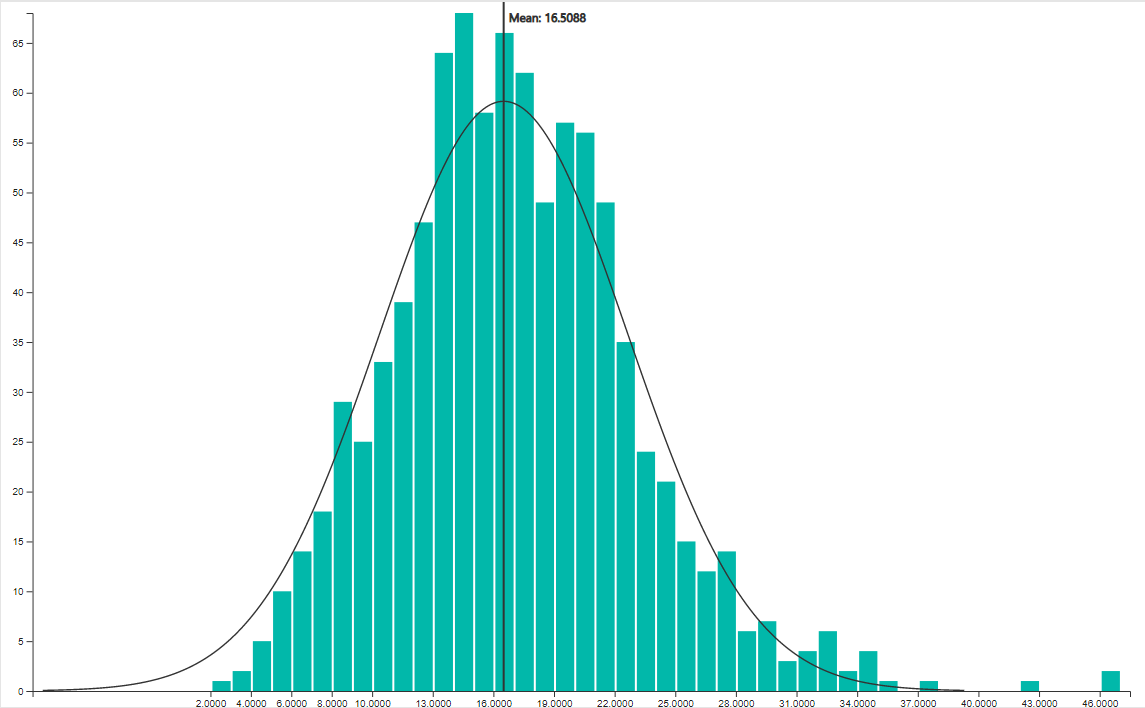
\includegraphics[width=0.75\textwidth]{assets/statistics/histogram.png}
    \caption{A histogram and the graph of the distribution of the samples}
\end{figure}

\begin{figure}[H]
    \centering
    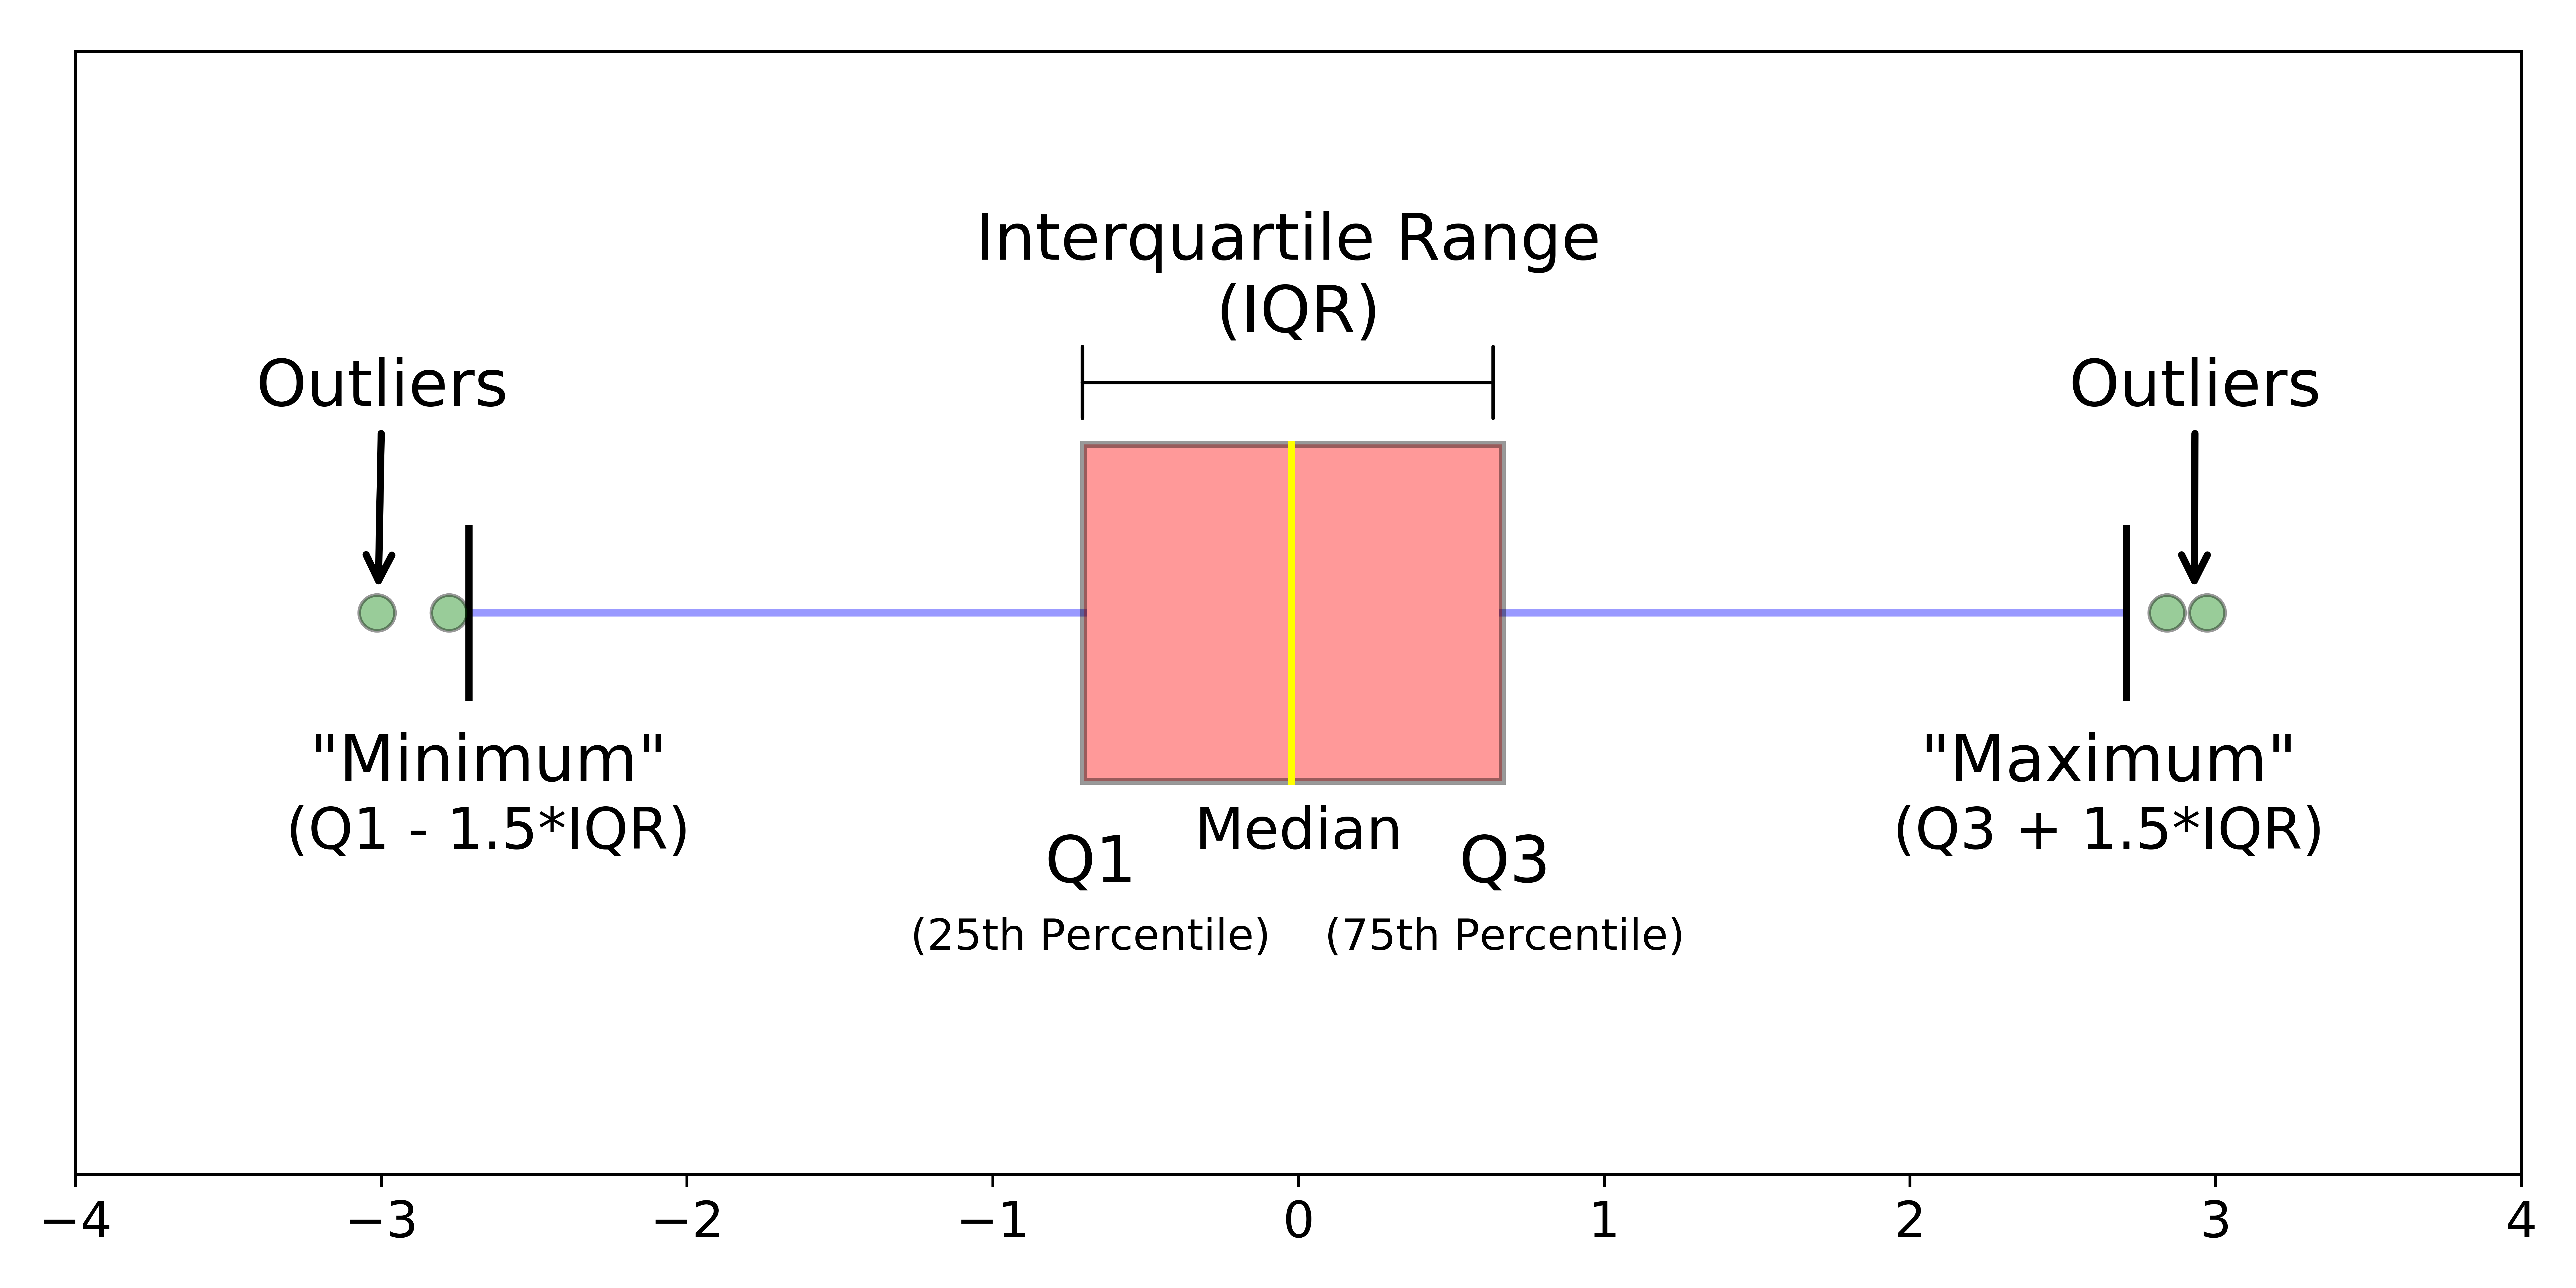
\includegraphics[width=0.75\textwidth]{assets/statistics/boxplot.png}
    \caption{A boxplot with indication on what the lines mean}
\end{figure}

Boxplots are very useful to check the symmetry of a sample.

\subsubsection{Location-Scale family of distributions}

\begin{definition}{Location-Scale family}{location-scale-family}
    Let $X$ be a random variable with distribution $F$ and $Y = a + bX$ with $b>0$.
    Then the distribution of $Y$ is
    \begin{equation}
        F_{a, b}(y) = F\left( \frac{y-a}{b} \right)
    \end{equation}
\end{definition}

\begin{example}{Normal distribution}{}
    $F$ is in the same location-scale family as the standard normal $\iff$ $F$ is a normal distribution
\end{example}

\subsubsection{Quantiles}

\begin{definition}{$\alpha$-quantiles}{alpha-quantiles}
    The $\alpha$-quantile of a distribution $F$ is given by
    \begin{equation}
        F^{-1}(\alpha) = \inf\{ x: F(x) \geq \alpha \}, \quad \alpha \in (0, 1)
    \end{equation}
\end{definition}

The quantile function of a location-scale family is
$F_{a, b}^{-1}(\alpha) = a + bF^{-1}(\alpha)$.

\begin{definition}{QQ-plot}{qq-plot}
    The QQ-plot for the realizations $x_1, \dots, x_n$ for a distribution function $F$ is a plot of the points
    \begin{equation}
        \left\{ \left( F^{-1}\left( \frac{i}{n+1} \right), x_i \right) : i = 1, \dots, n \right\}
    \end{equation}
    where $i$ is the order of the indices of $x_i$ such that they are in \textit{increasing order}.
\end{definition}

If the points $x_1, \dots, x_n$ come from $F$ then the points will approximately align to the $y = x$ line.
This is because we expect the sample quantile $x_i$ to be close to the theoretical quantile given by the formula.

\subsubsection{Correlation and independence}

As we know from Probability, we define the correlation coefficient as
\begin{equation}
    \rho_{A,B} = \frac{\cov(A, B)}{\sigma_A \sigma_B} \in [-1, 1]
\end{equation}

Recall that independence implies $\rho = 0$, but not viceversa (except for the normal distribution).

\begin{definition}{Sample correlation coefficient}{sample-correlation-coeff}
    Consider a sample of pairs $(X_1, Y_1), \dots, (X_n, Y_n)$.
    Then we define the sample correlation coefficient as
    \begin{equation}
        r_{X, Y} = \frac{\sum^n_{i = 1} (X_i - \bar{X})(Y_i - \bar{Y})}{(n-1)\sqrt{S^2_X} \sqrt{S^2_Y}}
    \end{equation}
\end{definition}

In the definition we use the following notation:
\begin{itemize}
    \item $\bar X$ is the sample mean
    \item $\sqrt{S^2_X}$ is the sample variance
\end{itemize}

We observe the following from $r_{X, Y}$:
\begin{itemize}
    \item $r_{X, Y} \in [-1, 1]$.
    \item If $r_{X, Y} = 1$ all the samples lie on the line $y = \bar y + \frac{S_y}{S_x}(x-\bar x)$.
    \item If $r_{X, Y} = -1$ all the samples lie on the line $y = \bar y - \frac{S_y}{S_x}(x-\bar x)$.
    \item If $X_1, \dots, X_n$ and $Y_1, \dots, Y_n$ are independent then $r_{X, Y}$ will be close to $0$.
\end{itemize}

Graphically we can observe correlation or independence using \textbf{scatter plots}: if the graph of $\{ (x_i, x_{i+1}) : i = 1, \dots, n-1 \}$ should show not much of a structure if the samples are independent.

\subsection{Estimation}

Estimation is the process of finding the best fitting distribution from the statistical model.

Suppose the model depends on an unknown parameter $\theta \in \Theta$:
\begin{equation}
    \mathcal M = \{ P_\theta : \theta \in \Theta \}
\end{equation}
Now we assume that $X = (X_1, \dots, X_n)$ has distribution $P_\theta$ for some $\theta \in \Theta$.
Then we want to find the $\theta$ that makes $P_\theta$ best fit the observed data.
We call this the \emph{true value of $\theta$}.
Sometimes it is even useful to compute the true value of some $g(\theta)$.

\begin{definition}{Estimator}{estimator}
    An \emph{estimator} is a random vector $T(X)$ that depends only on the observation $X$.

    The corresponding \emph{estimate} for a realization $x$ is $T(x)$.
\end{definition}

Note that estimators \emph{do not} depend on $\theta$.
The estimate will give us our value of $\theta$.

First, lets define some notation:
\begin{itemize}
    \item $T$ is the estimator $T(X)$.
    \item $t$ is the estimate $T(x)$.
    \item $\hat \theta$ is used for both the estimator and estimate of a unknown $\theta$ of interest
\end{itemize}

We could use as an estimator the distance between $T$ and $g(\theta)$
\begin{equation}
    \norm{T - g(\theta)}
\end{equation}

We want this difference to be as small as possible, that is, to be as concentrated as possible towards $0$.
Since $\norm{T - g(\theta)}$ is a random variable we can consider the one more concentrated around $0$.

\newcommand{\MSE}{{\operatorfont MSE}}

\begin{definition}{Mean squared error}{mean-squared-error}
    The mean squared error MSE of an estimator $T$ for the value of $g(\theta)$ is defined as
    \begin{equation}
        \MSE(\theta, T) = E_\theta\left(\norm{T - g(\theta)}^2\right)
    \end{equation}
    where $E_\theta$ is the expectation of $P_\theta$
\end{definition}

\begin{proposition}{MSE decomposition}{mse-decomposition}
    If a $T$ is real-valued estimator we can decompose the $\MSE$ as
    \begin{equation}
        \MSE(\theta, T) = V_\theta(T) + (E_\theta(T) - g(\theta))^2
    \end{equation}
\end{proposition}
\begin{proof}
    \begin{align}
        E_\theta\left((T - g(\theta))^2\right) & = E_\theta\left((T -E_\theta(T) + E_\theta(T) - g(\theta))^2\right)                                                            \\
                                               & = E_\theta(T-E_\theta(T))^2 - 2E_\theta(T-E_\theta(T))(E_\theta(T) - g(\theta)) + \cancel{E_\theta}(E_\theta(T) - g(\theta))^2 \\
                                               & = V_\theta(T) - 2 (E_\theta(T) - g(\theta)) \cancelto{0}{E_\theta(T-E_\theta(T))} - (E_\theta(T) - g(\theta))^2                \\
                                               & = V_\theta(T) - (E_\theta(T) - g(\theta))^2
    \end{align}
\end{proof}

We say that an estimator is \emph{biased} if it's expectation is not centered around $g(\theta)$.

\subsubsection{Maximum likelihood estimator}

\begin{definition}{Likelihood function}{likelihood-function}
    Let $X$ be a random vector with pdf $p_0$ that depends on a parameter $\theta \in \Theta$.
    For a fixed $x$ the likelihood function is defined as
    \begin{equation}
        \theta \mapsto L(\theta, x) = p_\theta(x)
    \end{equation}
\end{definition}

\begin{lemma}{IID variables}{}
    If $X_1, \dots, X_n$ IID then
    \begin{equation}
        L(\theta; X_1, \dots, X_n) = \prod_{i = 1}^{n} L(\theta, X_i)
    \end{equation}
\end{lemma}

\begin{definition}{Maximum likelihood estimator}{}
    The maximum likelihood estimate of $\theta$ is the value $T(x) \in \Theta$ that maximizes the likelihood function $L(\theta; x)$.

    The maximum likelihood estimator is $T(X)$.
\end{definition}

An useful trick we can use to find the maximum likelihood estimate is to apply the $\log$ to the likelihood function.
In this way we are left to deal with sums and not products (by the properties of logarithms), and, since $\log$ is monotone, the maximum of the transformation will be the maximum of the original function.

We will call \textbf{score function} the derivative of the likelihood function (or its log transformation).

The idea behind the likelihood function is that this is a function that, given an observation $x$, gives us the probability that the $\theta$ we chose was good.

\begin{example}{Exponential distribution}{mle-exponential}
    Let $X = (X_1, \dots, X_n)$ be a sample from the exponential distribution with unknown parameter $\lambda \in (0, \infty)$.

    The sample space is
    \begin{equation}
        \mathcal{M} = \{ p_\lambda(x) = \lambda e^{-\lambda x}, x > 0 \}
    \end{equation}
    then we compute the pmf
    \begin{equation}
        p_\lambda (x_1, \dots, x_n) = \prod_{i = 1}^n (\lambda e^{-\lambda x}) = \lambda^n e^{-\lambda \sum_{i = 1}^n x_i}
    \end{equation}
    therefore, the likelihood function is
    \begin{equation}
        L(\lambda; x_1, \dots, x_n) = \lambda^n e^{-\lambda \sum_{i = 1}^n x_i}
    \end{equation}

    Now we want to maximize $L$ but it is easier to take the $\log$ first:
    \begin{equation}
        l(\lambda; x_1, \dots, x_n) = n\log(\lambda) + \lambda \sum_{i = 1}^n x_i
    \end{equation}
    and by differentiating we get the score equation to be
    \begin{equation}
        \frac{n}{\lambda} - \sum_{i = 1}^{n} x_i = 0
        \implies \hat \lambda = \frac{1}{\bar{x}}
    \end{equation}

    The last thing we are left to do is to make sure this is a maximum point, therefore we have to take the second derivative:
    \begin{equation}
        \dv{}{\lambda} \left( \frac{n}{\lambda} - \sum_{i = 1}^{n} x_i \right) = -\frac{n}{\lambda^2} < 0
    \end{equation}
    hence it is indeed a point of maximum.

    We conclude that $\hat \lambda = \frac{1}{\bar{x}}$ is the maximum likelihood estimate.
\end{example}

\begin{example}{Coin tosses}{mle-bernoulli}
    A coin with unknown $p = P(\text{HEAD})$ is tossed $n = 100$ times and shows heads $60$ times.
    Intuitively we would say that $p = 0.6$.
    Let's check it.

    We have that $X_1, \dots, X_n$ IID $\sim \Bernoulli(p)$ therefore
    \begin{align}
        L(p; X_1, \dots, X_n)         & = \prod_{i = 1}^n \left( p^{X_i} (1 - p)^{1-X_i} \right)   \\
                                      & = p ^{\sum_{i = 1}^n X_i} (1-p) ^{\sum_{i = 1}^n (1- X_i)} \\
                                      & = p^{n \bar X} (1-p)^{n(1-\bar{X})}                        \\
        l(p; X_1, \dots, X_n)         & = n \bar X \log p + n(1- \bar{X}) \log(1-p)                \\
        \dv{l(p; X_1, \dots, X_n)}{p} & = \frac{n \bar x}{p} - \frac{n(1-\bar{x})}{1-p}
    \end{align}

    Now we have our score function that we want to maximize:
    \begin{align}
        \max_p                           & \frac{n \bar x}{p} - \frac{n(1-\bar{X})}{1-p}                             \\
                                         & \implies \frac{\cancel {n} \bar X}{p} = \frac{\cancel{n}(1-\bar{X})}{1-p} \\
                                         & \implies \bar{X} (1-p) = p (1-\bar X)                                     \\
                                         & \implies \bar{X} -\cancel{p\bar{X}} = p -\cancel{p\bar{X}}
        \implies \hat p = \bar{X}                                                                                    \\
        \dv[2]{l(p; X_1, \dots, X_n)}{p} & = -\frac{n \bar{X}}{p^2} - \frac{n(1-\bar X)}{(1-p)^2} < 0                \\
                                         & \implies \hat p \text{ is the MLE.}
    \end{align}
    which indeed corresponds to the intuitive result.
\end{example}

\begin{example}{Uniform distribution}{mle-uniform}
    Let $X_1, \dots, X_n \stackrel{\text{IID}}{\sim} \Uniform(0,\theta)$ with $\theta$ unknown.

    \begin{align}
        L(\theta; X_1, \dots, X_n) & = \prod_{i = 1}^n \frac{1}{n} 1_{[0, \theta]}(x_i)                \\
                                   & =\theta^{-n} \prod_{i = 1}^n 1_{[x_i, \infty)} (\theta)           \\ % TODO: explain this better
                                   & = \theta^{-n} 1_{[x_1; \infty) \cap \dots \cap [x_n; \infty)}     \\
                                   & = \theta^{-n} 1_{\left[\max_n \{x_1, \dots, x_n\}; \infty\right)}
    \end{align}

    Now we can look at the two cases of the indicator function and we see that the maximum occurs at $\hat \theta = \max_n x_n$.
\end{example}

\begin{example}{Normal distribution}{mle-normal}
    Let $X_1, \dots, X_n \stackrel{\text{IID}}{\sim} \Normal(\mu,\sigma^2)$ with $\mu,\sigma^2$ unknown.

    \begin{align}
        L(\mu,\sigma^2; X_1, \dots, X_n)                   & = \prod_{i = 1}^n \frac{1}{\sqrt{2 \pi \sigma^2}} e^{-\frac{(X_i - \mu)^2}{2 \sigma^2}}                                 \\
                                                           & = (2 \pi \sigma^2)^{-\frac{n}{2}} e^{- \sum_{i = 1}^n \frac{(X_i - \mu)^2}{2 \sigma^2}}                                 \\
        l(\mu,\sigma^2; X_1, \dots, X_n)                   & = -\frac{n}{2}\log(2 \pi \sigma^2) - \sum_{i = 1}^n \frac{(X_i - \mu)^2}{2 \sigma^2}                                    \\
        \pdv{l(\mu,\sigma^2; X_1, \dots, X_n)}{\mu}        & = \cancel{-1 }\cdot \cancel{-} \sum_{i = 1}^n \frac{\cancel{2}(X_i - \mu)}{\cancel{2} \sigma^2}  \label{eq:mle-n-seq-1} \\
        \pdv{l(\mu,\sigma^2; X_1, \dots, X_n)}{(\sigma^2)} & = -\frac{n}{2 \sigma^2} + \sum_{i = 1}^n \frac{(X_i - \mu)^2}{2 \sigma^4} \label{eq:mle-n-seq-2}
    \end{align}

    Now we have that \cref{eq:mle-n-seq-1} and \cref{eq:mle-n-seq-2} are our score functions which we want to maximize.
    \begin{align}
        \sum_{i = 0}^{n} \frac{(X_i - \hat \mu)}{\sigma^2} = 0                      & \implies \hat \mu = \bar X                                            \\
        -\frac{n}{2 \sigma^2} + \sum_{i = 1}^n \frac{(X_i - \mu)^2}{2 \sigma^4} = 0 & \implies \hat{\sigma}^2 = \frac{1}{n} \sum_{i = 1}^n (X_1 - \bar X)^2
    \end{align}
    where we substituted the first result into the second equation in order to solve it.
    It can be shown that $\hat \mu$ and $\hat \sigma$ are maximizers but we'll omit it here.

    We see that $\hat \mu$ is unbiased while $\hat \sigma ^2$ is.
\end{example}

\subsubsection{Method of moments estimators}

\begin{definition}{Moment and sample moment}{moment-sample-moment}
    Let $X \sim p_\theta$. The $j$-th moment of $X$ is given by
    \begin{equation}
        E_\theta(X^j),
    \end{equation}
    assuming the expectation exists.

    Similarly, the $j$-th sample moment of $X_1,\dots, X_n$ IID random variables is defined as
    \begin{equation}
        \bar{X_j} = \frac{1}{n} \sum_{i = 1}^n X_i^j \convas E_\theta(X^j)
    \end{equation}
    by the law of large numbers.
\end{definition}

The idea is that we compute the moment and the sample moment, then we choose the parameter such that the moment and the sample moment coincides.
This is very simple and most times it coincides with the MLE.
We repeat the process until the $k$-th moment, where $k$ is the smallest number such that the system has a unique solution.

\begin{example}{Common distributions}{}
    \begin{itemize}
        \item \emph{Exponential}: same result as MLE;
        \item \emph{Uniform}: $\hat \theta = 2 \bar X$ which is a worse result than the MLE.
    \end{itemize}
\end{example}

Note that in this way we are summarizing the distribution in $k$ values. A best method is to find the $\hat \theta$ that minimizes the distance between the two moments.
For example, if we use $l$ moments, we define the \emph{generalized method of moments} as
\begin{equation}
    \sum_{i = 0}^l \left( \frac{1}{n} \sum_{i = 0}^n X^j_i - E(X_i^j) \right)^2
\end{equation}
or, even more generally, for some fixed $g_1, \dots, g_n$,
\begin{equation}
    \sum_{i = 0}^l \left( \frac{1}{n} \sum_{i = 0}^n g_j(X_i) - E(g_j(X_i)) \right)^2
\end{equation}

\section{Bayesian statistics}

\subsection{Introduction}

This is the oldest method of constructing estimators.
The main idea is that there is no unique true parameter, every parameter has it's own probability.
The main problem of this strategy is that there are problems with computing the result (except for simple cases).
Nowadays this method is widely used in combination with computer-based simulations.

\begin{definition}{Bayesian model}{bayesian-model}
    A statistical model in bayesian statistics is
    \begin{equation}
        \mathcal M = \{ p_\theta : \theta \in \Theta \}
    \end{equation}
    and a \emph{prior distribution} $\pi$ on the parameter space $\Theta$.
\end{definition}

Differently from before, $\theta$ is seen as a \emph{random variable}, not an unknown.
The choice of $\pi$ is driven by subjective belief, based on experience and likelihood of different values of $\theta$.
After observing the data we \emph{update our believes} by computing the posterior distribution.

\begin{definition}{Bayes risk}{bayes-risk}
    The Bayes risk of an estimator $T$ for a real-valued parameter $g(\theta)$ is defined as
    \begin{equation}
        R(\pi; T) = \int_\Theta E_\theta[(T-g(\theta)^2)] \pi(\theta) \dd{\theta}
    \end{equation}
\end{definition}
This is pretty much the equivalent of the MSE for bayesian models.

\begin{definition}{Bayes estimator}{bayes-estimator}
    The Bayes estimator with respect to the prior density $\pi$ is the estimator $T$ that minimizes $R(\pi; T)$.
\end{definition}

\begin{theorem}{Bayes estimator - first version}{bayes-estimator-v1}
    The Bayes estimator for $g(\theta)$ w.r.t. the prior density $\pi$ is
    \begin{equation}
        T(x) = \frac{\int_\Theta g(\theta) p_\theta(x)\pi(\theta) \dd{\theta}}{\int_\Theta g(\theta) \pi(\theta) \dd{\theta}}
    \end{equation}
\end{theorem}

\begin{proof}
    Start by the definition of bayesian risk and plug in the definition of expectation.
    \begin{align}
        R(\pi; T) & = \int_\Theta E_\theta[(T-g(\theta)^2)] \pi(\theta) \dd{\theta}                                               \\
                  & = \int_\Theta \left(\int_X (T-g(\theta))^2 p_\theta(x)\dd{x} \right) \pi(\theta) \dd{\theta}                  \\
                  & \stackrel{\text{fubini}}{=} \int_X \int_\Theta (T(x) - g(\theta))^2 p_\theta(x) \pi(\theta) \dd{\theta}\dd{x}
    \end{align}

    The goal is to minimize for all $x$. We can just minimize the inside integral as that will result in the minimization of the whole expression.
    \begin{align}
        \argmin & \int_\Theta (T(x) - g(\theta))^2 p_\theta(x) \pi(\theta) \dd{\theta}                                                                                                                    \\
                & = T^2(x) \int_\Theta p_\theta(x) \pi(\theta) \dd{\theta}- 2T(x) \int_\Theta g(\theta) p_\theta(x) \pi(\theta) \dd{\theta} + \int_\Theta g^2(\theta) p_\theta(x) \pi(\theta) \dd{\theta}
    \end{align}

    Now we take the derivative w.r.t. $T(x)$ and set it equal to zero:
    \begin{gather}
        \cancel 2 T(x) \int_\Theta p_\theta(x) \pi(\theta) \dd{\theta}- \cancel 2 \int_\Theta g(\theta) p_\theta(x) \pi(\theta) \dd{\theta} = 0 \\
        \implies T(x) = \frac{\int_\Theta p_\theta(x) \pi(\theta) \dd{\theta}}{\int_\Theta g(\theta) p_\theta(x) \pi(\theta) \dd{\theta}}
    \end{gather}
\end{proof}

\begin{definition}{Posterior distribution}{posterior-distribution}
    The posterior distribution of $\bar \Theta$ conditionally on $X = x$ is
    \begin{equation}
        p_{\bar \Theta | X = x} (\theta) = \frac{p_\theta(x) \pi(\theta)}{\int_\Theta p_\theta(x) \pi(\theta) \dd{\theta}}
    \end{equation}
\end{definition}

We say that the the prior and the posterior distribution are \emph{conjugated} if they belong to the same family of distributions.

Now we can rewrite \Cref{thm:bayes-estimator-v1} by substituting this new definition:

\begin{theorem}{Bayes estimator - second version}{bayes-estimator-v2}
    The Bayes estimator for $g(\theta)$ w.r.t. the prior density $\pi$ is
    \begin{equation}
        T(x) = \int_\Theta g(\theta) p_{\bar \Theta | X = x} (\theta) \dd{\theta} = E[g(\bar \Theta) | X = x]
    \end{equation}
\end{theorem}

\subsection{Estimation}

We can use an estimator $t = T(x)$ to estimate the value of $\theta$ but usually our estimate will be wrong, the point estimate $t$ will generally differ from $\theta$.
In this section we will try to quantify the difference between $t$ an $\theta$ and, if $\theta \in \R$, find an \emph{interval estimate} $[L(x), R(x)]$ where $\theta$ has a high probability of lying.

\begin{definition}{Confidence region}{confidence-region}
    Let $X$ be a random variable depending on a parameter $\theta \in \Theta$.
    Let $G_X \in \mathcal P(X)$.
    The map $X \mapsto G_X$ is a confidence region for $\theta$ of confidence level $1-\alpha$ if
    \begin{equation}
        P_\theta(G_X \ni \theta) \geq 1- \alpha \quad \forall \theta \in \Theta
    \end{equation}
    where usually $\alpha$ is small.
\end{definition}

We note the following facts:
\begin{enumerate}
    \item $G_X$ is a stochastic (i.e. random) subset of $\Theta$ as it depends on a random variable $X$; meanwhile $\theta$ is a fixed number.
    \item The event $\{ G_X \ni \theta \}$ has as random object $G_X$.
    \item Given a realization $X = x$, also $G_X$ realizes to $G_x$ which is therefore not random anymore.
    \item Since $G_x$ and $\theta$ are both fixed, then either $\theta \in G_x$ or $\theta \notin G_x$.
\end{enumerate}

In bayesian statistics we interpret the true value of $\theta$ as the realization of $\bar \Theta$.
In this context we can make a statement about the random parameter \emph{after} the realization $X = x$, of the type
\begin{equation}
    P(\bar \Theta \in G_X \mid X = x)
\end{equation}
and we can determine this probability by the posterior distribution of $p_{\bar \Theta \mid X = x}$.

If we focus on $\theta \in \R$ we have that confidence regions are usually intervals of the form $G_X = [R(X), L(X)]$.
If the interval is centered around the point estimate $t$ then it is called \emph{symmetric} and we write $\theta = t \pm \eta$ with $\eta = [R(x) - L(x)]/2$.

\begin{example}{Normal distribution}{}
    Let $X_1, \dots X_n$ be a sample from the normal distribution $\Normal(\theta, \sigma^2)$, with unknown mean $\theta$ and known variance $\sigma^2$.
    Find a confidence interval for $\theta$ of level of confidence $1-\alpha$.
\end{example}

\begin{proof}[Solution]
    TODO: vedi appunti bea, che minchia è $\xi$?
\end{proof}

\subsubsection{Pivots}

\begin{definition}{Pivot}{pivot}
    A pivot is a function $T(X, \theta)$ whose probability distribution does not depend on $\theta$ or any other parameter.
\end{definition}

Note that for a pivot $T(X, \theta)$ the probability $P_\theta(T(X, \theta) \in B)$ is not a function of $\theta$.

For the normal distribution a pivot is
\begin{equation}
    T(X, \theta) = \frac{\bar X - \theta}{\sigma /\sqrt{n}}
\end{equation}
which is distribution according to the standard normal.

We can define a confidence region for a pivot as well.
For eery $B$ such that $P_\theta(T(X, \theta) \in B) \geq 1- \alpha$, the set
\begin{equation}
    \{ \theta \in \Theta : T(X, \theta) \in B \}
\end{equation}
is the confidence region for $\theta$ of confidence level $1- \alpha$.

\begin{example}{Uniform distribution}{}
    Let $X_1,...,X_n$ be a sample from the uniform distribution $\Uniform(0,\theta)$, with $\theta$ unknown.
    Find a confidence interval for $\theta$ of level of confidence $1 - \alpha$.
\end{example}

\begin{proof}[Solution]
    TODO: chiedere a bea :D
\end{proof}

\end{document}
